\documentclass[twocolumn]{autart}

%% DOI and ARXIV Commands for Bib Files
% Written by Daniel Herber
% -----------------------------------------------
% one option is to use the 'note' field with this command
% -----------------------------------------------
% for example, if your doi is 10.2514/1.J052182
% then for the citation for the reference in your bib file, use
% note = "\doi{10.2514/1.J052182}",
% -----------------------------------------------
% for example, if your arxiv number is 0706.1234
% then for the citation for the reference in your bib file, use
% note = "\arxiv{0706.1234}",

% requires hyperref package for \href command
\usepackage{hyperref}

% doi command (use in bib file)
\newcommand{\doi}[1]{{doi:~\href{http://doi.org/#1}{#1}}\rmFullStop}

% arXiv command (use in bib file)
\newcommand{\arxiv}[1]{{arXiv:\href{https://arxiv.org/abs/#1}{#1}}\rmFullStop}

% command to remove full stop if the next character
\newcommand*{\rmFullStop}{\rmifnextchar{.}{}{}}

% command to check the next character and replace if present
% \rmifnextchar{X}{[removed text]}{[no X text]}
% if X is the next character, then it is removed and [removed text] is inserted
% otherwise, the character is not removed and [no X text] is inserted
% based on http://tex.stackexchange.com/questions/72827
\makeatletter
\newcommand{\rmifnextchar}[3]{%
  \begingroup
  \ltx@LocToksA{\endgroup#2}%
  \ltx@LocToksB{\endgroup#3}%
  \ltx@ifnextchar{#1}{%
    \def\next{\the\ltx@LocToksA}%
    \afterassignment\next
    \let\scratch= %
  }{%
    \the\ltx@LocToksB
  }%
}
\makeatother
%\RequirePackage{doi}
\usepackage[
	pdftitle={SPARQLing Ogham Stones - Blogpost},
	pdfsubject={SPARQLing Ogham Stones - Blogpost},
	pdfauthor={Sophie Charolotte Schmidt, Florian Thiery},
	pdfkeywords={best practices, data, interdisciplinarity, Ogham, repositories, Wikidata}
]{hyperref}

\usepackage{graphicx}          % Include this line if your 
                               % document contains figures,
%\usepackage[dvips]{epsfig}    % or this line, depending on which
                               % you prefer.
\usepackage{verbatimbox}

\begin{document}

\begin{frontmatter}
%\runtitle{Insert a suggested running title}  % Running title for regular 
                                              % papers but only if the title  
                                              % is over 5 words. Running title 
                                              % is not shown in output.

\title{SPARQLing Ogham Stones - Blogpost}
                                               

\author[SCS]{Sophie C. Schmidt}
\author[FT]{Florian Thiery}

\address[SCS]{ORCID: 0000-0003-4696-2101, Research Squirrel Engineers}
\address[FT]{ORCID: 0000-0002-3246-3531, Research Squirrel Engineers}

          
\begin{keyword}                             
best practices, data, interdisciplinarity, Ogham, repositories, Wikidata.
\end{keyword}

\begin{abstract}                         

This is a blogpost from Archaeoloinformatics.net\cite{schmidt_sparqling_2020} .

\end{abstract}

\end{frontmatter}

Together with Florian Thiery I gave a talk on a side project by the Research Squirrel Engineers, a working group of Research Software Engineers. Our aim in this project is to digitize a catalogue on Ogham stones and put it online in a linked and open way. At the Graph Technologies in the Humanities conference we were invited to present our work. Here is a short version.

Do you hate copying analog tables and catalogues as much as we do? We hate it with passion and believe we should be way past such useless tasks by now. I mean, it takes such a lot of time, is tedious and everyone doing it for a longer time is prone to committing mistakes. It just happens, that’s life. I mean, of course, if there’s an old data set, that’s only available in print, we have to digitize it in some way. But people are digitizing stuff that has been copied by somebody else already! Double the time invested in this horrible mind-numbing task…

And do you agree it is very annoying if there is information on the web that is inaccessible? I mean, seriously. A database without an API? No possibilities of (dynamically) downloading anything? Why would you put data online if you don’t want people to use it?? This is so 1990’s… (no offense to databases this old :-) )

Do you, by any chance, think that data should be findable? So, if you find a hint in a database, that there’s another database out there, that may have some more info than this one, would you like to be able to access that data set easily and find the correct ID for the entry you’ve just studied? So you can add it to your database, if needed?

Yes?

Yes, me too.

And there’s a word for all of these things. I am talking about Linked Open Data.

\begin{figure}[!htb]
\begin{center}
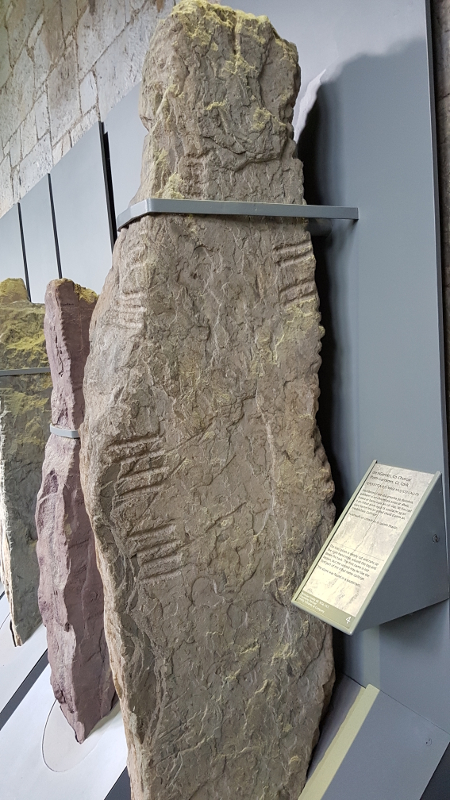
\includegraphics[width=6cm]{UCC_Stone_4.jpg}
\caption{UCC Stone Corridor, Stone 4, CIIC 81, Florian Thiery [CC BY 4.0] via Wikimedia Commons}
\label{rq1}
\end{center}
\end{figure}

Ogham stones are stones that have been erected mostly in Ireland during the 4th to 9th century AD. They are inscribed with the Ogham script which is an alphabet that was developed for the (proto-) Irish language and relies on strokes along a ridge to form the letters. Mostly the information given on these stones is something along the lines of “for Tom, son of Paul” or “for Peter son of the tribe of the Toms”. We don’t know whether they were grave markers, memorials or meant to indicate land ownership. But they are really quite interesting, because they are the earliest evidence of the Irish language and tell us something about tribal and familial structures in a time where we don’t have many written sources yet.

If you want to study the stones, you have to use a number of printed publications as offline sources. You can use the database of the Celtic Inscribed Stones Project, which has been put up online about 20 years ago and is not very accessible according to modern standards (you may click through the entries). There is the Historic Environment Viewer by the Irish Heritage Management, which is great, because you can download spatial information. Also the Ogham 3D Project has a number of digitized information on those stones that they scanned. But those different data sets are not linked at all. You can’t easily go from one to another and compare information. Not optimal.

So we took the catalogue of Ogham stones by Macálister 1945 and started with digitizing information mostly concerned with the location. Macálister used townlands and baronies as main indication where stones were found. We identified these and linked them to the open street map IDs, as well as to other spatial information, e.g. district and parish in which they are located (info we found on townlands.ie). We are also working on incorporating information given in the CISP project (they gave us their database to re-use. Thank you, Kris Lockyear!), but that’s an ongoing process of mapping the data sets, this takes some time.

Now, our aim is to make this data available for everyone. There are several ways of putting data online in such a way. We decided to use Wikidata, as it is a growing repository for all kinds of information. It is the central storage for structured data of Wikimedia projects. It is a available under a free license (CC 0), multilingual, accessible to humans and machines (GUI / API / SPARQL), exportable using standard formats (JSON, RDF, XML) and interlinks to other open data sets on the LOD Cloud.

The “problem” with Wikidata is, that it uses a query language, that one needs to know to really access the content. Because we are sure there are a number of people who don’t know SPARQL, the Research Squirrels Martina and Florian developed the SPARQL unicorn. It’s the idea to create GUIs that make it easy for people to use Wikidata data. One is already working: the SPARQLing Unicorn QGIS plug-in! We also want to create an R package that might help people to further analyse Wikidata data.

So, it’s all work in progress, but we are getting there. We were offered some positive feedback and I’m glad people liked our idea of making data available for further use. Are you interested in more? Here are our slides and we will probably be add this paper to the graph conference publication. So, stay tuned!

\begin{ack}                               

\begin{figure}[!htb]
\begin{center}

\includegraphics[width=8cm]{rse_logo.png}
\caption{Research Squirrel Engineers}
\label{rq1}
\end{center}
\end{figure}

\textbf{The Research Squirrel Engineers}

http://squirrel.link

\textit{Sophie Charlotte Schmidt}

\textit{Martina Trognitz}

\textit{Florian Thiery}

\textit{Timo Homburg}

\end{ack}

\bibliographystyle{IEEEtran}
\bibliography{autosam}

\end{document}